


 
    \section{Cycles of science}
    \label{cycles}

        How it all fits together.



        \subsection{Improvements to observatories}
        \label{observatories_better}

            Enhancements like enhanced/advanced LIGO and squeezing.

        \subsection{Understanding instruments}
        \label{instrumental_understanding}

            ....necessitate detector characterization, like scans and filters

        \subsection{Refining data}
        \label{data_refinements}

            ....automated feedforward filters yield own enhancements

        \subsection{Searching deep-space}
        \label{searching_space}

            ...TwoSpect and other searches benefit

        \subsection{Reaching out, looking up}
        \label{reaching_out}

            ...Outreach makes research accessible to public.

    \section{Scientific merit: filtering and analysis}
    \label{merit}

        Core projects.

        \subsection{Feedforward improvement to LIGO data}
        \label{feedforward_end}

            Evaluate success of feedforward.

        \subsection{TwoSpect directed search for neutron stars in binary systems}
        \label{TwoSpect_end}

            ...and TwoSpect-directed.

            One thought that might develop into something more fruitful is as follows.

            Someday deconvolve, maybe Bayesian, the skymaps and parameter space spread of TwoSpect with simulation to understand what we are really seeing. Cannot do all templates in paramter space, but only need a few to compare -- in a way, it already does.

    \section{Entering the advanced detector era}
    \label{advanced_detector_era}

        Advanced LIGO: how much better can we do?

    \section{Vision of a dark sky}
    \label{dark_sky}

\begin{figure}
\begin{center}
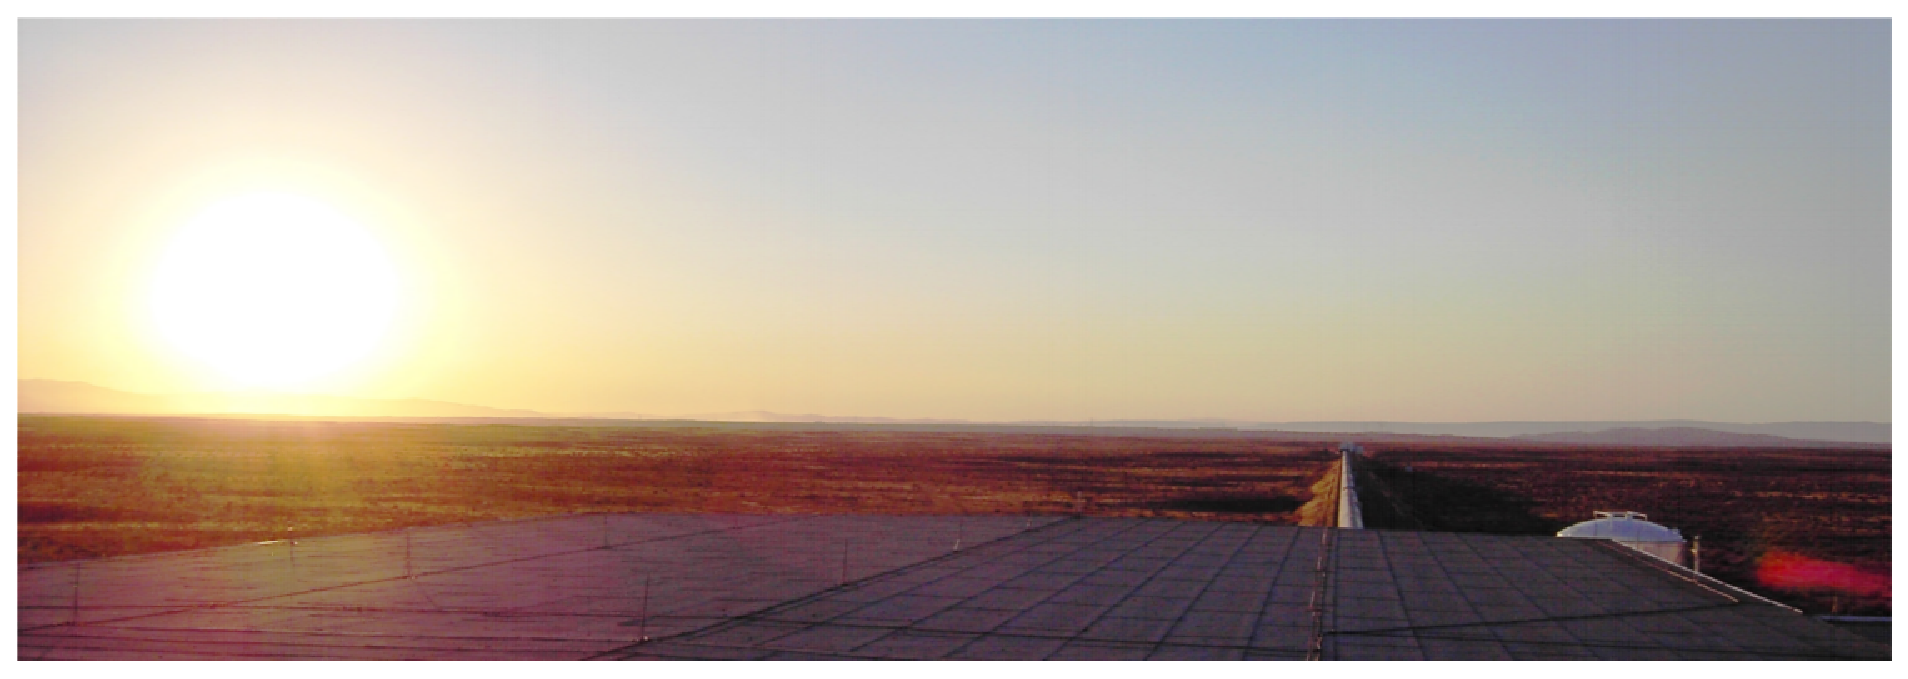
\includegraphics[height=50mm,width=148mm]{LIGOpanoramasmall.eps}
\caption{LIGO Hanford Observatory sunset, inital detector era. Photo by author. Like the Hanford desert wiped clean by the Missoula floods, the gravitational wave sky may relate cosmic tales of cataclysm and rebirth in the distant past.}
\label{LIGO_panorama_small}
\end{center}
\end{figure}

        Why GW astronomy at all? What could be out there?

        Gravity is the universe. At the dawn of the twenty-first century, the Standard Model of physics, and quantum field theory in general, can be studied on curved spacetime, but the spacetime itself remains scarcely better understood than when Einstein first proposed it general relativity. After almost a century, the fabric of the universe is still stiff and unyielding of its secrets. Gravitational wave astronomy will be the first science to unravel that fabric. 

        In this thesis, we have made inroads to this new astronomy. Superficially seperate, the common thread is the pursuit of fundamental issues by skillful choice of perspective. 
With squeezing, the optical experimenter views a gravitational wave interferometer as a quantum system and sees how fluctuations in the vacuum, not just in the laser, create noise -- which can be cancelled with a beam of no-light.
With feedforward, the noise due to intrinsic couplings between the interferometer servos is found by coherence in the frequency domain -- and cancelled with subtraction that can take place either in real-time or long afterward.
With TwoSpect, signals buried beneath noise are uncovered by comparing multiple instruments -- cancelling noise, in effect, with the build-up of signal in other observatories.
Communicating these advances to a wider world is the final question of fundamental issues and choice of perspective.
Gravitational wave observations have not yet seen a signal, yet we find ways to make our research meaningful.

Until we can see in gravity, we will be ignorant to the range of forces present in the cosmos. From the windswept, tumbleweed-coated plains of Hanford and the primordial swamps of Livingston may emerge our first visions of this thus-far dark sky. From it may come unexpected sources. Even if, though, we see only what we imagine will be seen, the insight into the hearts of neutron stars, the explosions of giant suns, the collisions of black holes, and the earliest, as-yet opaque instants of the universe will be wonder enough. The author can only hope to have contributed in some small way to this project. 

  
% Document Control Center, DCC, information:
% Directed searches for continuous gravitational waves from spinning neutron stars in binary systems 
% LIGO DCC-P1400102

%        -------------------------------------
%
%	The following is an example of using the commands \textit{ref}
%	and \textit{label}. With these commands theorems, chapters,
%	sections and figurres can be labeld with names in the tex file
%	and then refered to by these names in later tex files. In
%	chapter~\ref{intro} we saw section~\ref{sample_section} or
%	theorem~\ref{sample_theorem}.
%
%	Lastly, here is how to include a figure. First generate an
%	encapsulated postscript file in xfig, adobe illustrator or
%	some other program. The specific commands are found in
%	\textit{chap2.tex}.
%
%        \begin{figure}[htb]
%        \centerline{ \epsfig{figure=sample.eps, 
%        height =  1.5 in}}
%        \caption{Sample Figure}
%        \label{sample_figure}
%        \end{figure}

